% This LaTeX was auto-generated from MATLAB code.
% To make changes, update the MATLAB code and export to LaTeX again.

\documentclass{article}

\usepackage[utf8]{inputenc}
\usepackage[T1]{fontenc}
\usepackage{lmodern}
\usepackage{graphicx}
\usepackage{color}
\usepackage{listings}
\usepackage{hyperref}
\usepackage{amsmath}
\usepackage{amsfonts}
\usepackage{epstopdf}
\usepackage{matlab}

\sloppy
\epstopdfsetup{outdir=./}
\graphicspath{ {./README_images/} }

\begin{document}

\matlabheading{NIfTI MRS import into MATLAB}

\begin{par}
\begin{flushleft}
This document aims to demonstrate how magnetic resonance spectroscopy data stored according \href{https://docs.google.com/document/d/1tC4ugzGUPLoqHRGrWvOcGCuCh_Dogx_uu0cxKub0EsM/edit}{to the proposed NIfTI MRS format specification} can be loaded into MATLAB.
\end{flushleft}
\end{par}

\begin{par}
\begin{flushleft}
First, clone the following two repositories into your MATLAB directory:
\end{flushleft}
\end{par}

\begin{par}
\begin{flushleft}
\href{https://github.com/wexeee/mrs_nifti_standard}{https://github.com/wexeee/mrs\_nifti\_standard} (example data)
\end{flushleft}
\end{par}

\begin{par}
\begin{flushleft}
\href{https://github.com/xiangruili/dicm2nii}{https://github.com/xiangruili/dicm2nii} (DICOM import/export tools)
\end{flushleft}
\end{par}

\begin{matlabcode}
% Find MATLAB path
pathMATLAB = userpath;

% Add data and DICOM tools
addpath(genpath([userpath filesep 'dicm2nii']));
addpath(genpath([userpath filesep 'mrs_nifti_standard']));
\end{matlabcode}

\begin{par}
\begin{flushleft}
Define the example filename we want to load
\end{flushleft}
\end{par}

\begin{matlabcode}
nifti_file = 'svs_preprocessed.nii.gz';
\end{matlabcode}

\begin{par}
\begin{flushleft}
Load the NIfTI file:
\end{flushleft}
\end{par}

\begin{matlabcode}
nii = nii_tool('load', nifti_file);
\end{matlabcode}

\begin{par}
\begin{flushleft}
The resulting \texttt{nii} struct contains the data array (\texttt{img}) , NIfTI header (\texttt{hdr)}, and the MRS header extension (\texttt{ext}):
\end{flushleft}
\end{par}

\begin{matlabcode}
nii
\end{matlabcode}
\begin{matlaboutput}
nii = 
    hdr: [1x1 struct]
    ext: [1x1 struct]
    img: [1x1x1x4096 single]

\end{matlaboutput}

\matlabheading{Complex time-domain data}

\begin{par}
\begin{flushleft}
The complex time-domain data is stored in the \texttt{img} array, with the first three dimensions being spatial x, y and z dimensions, and the fourth dimensions being time. We can plot the single stored SV FID:
\end{flushleft}
\end{par}

\begin{matlabcode}
fid = squeeze(nii.img);
plot(real(fid));
hold on
plot(imag(fid));
legend('real', 'imag');
hold off
\end{matlabcode}
\begin{center}
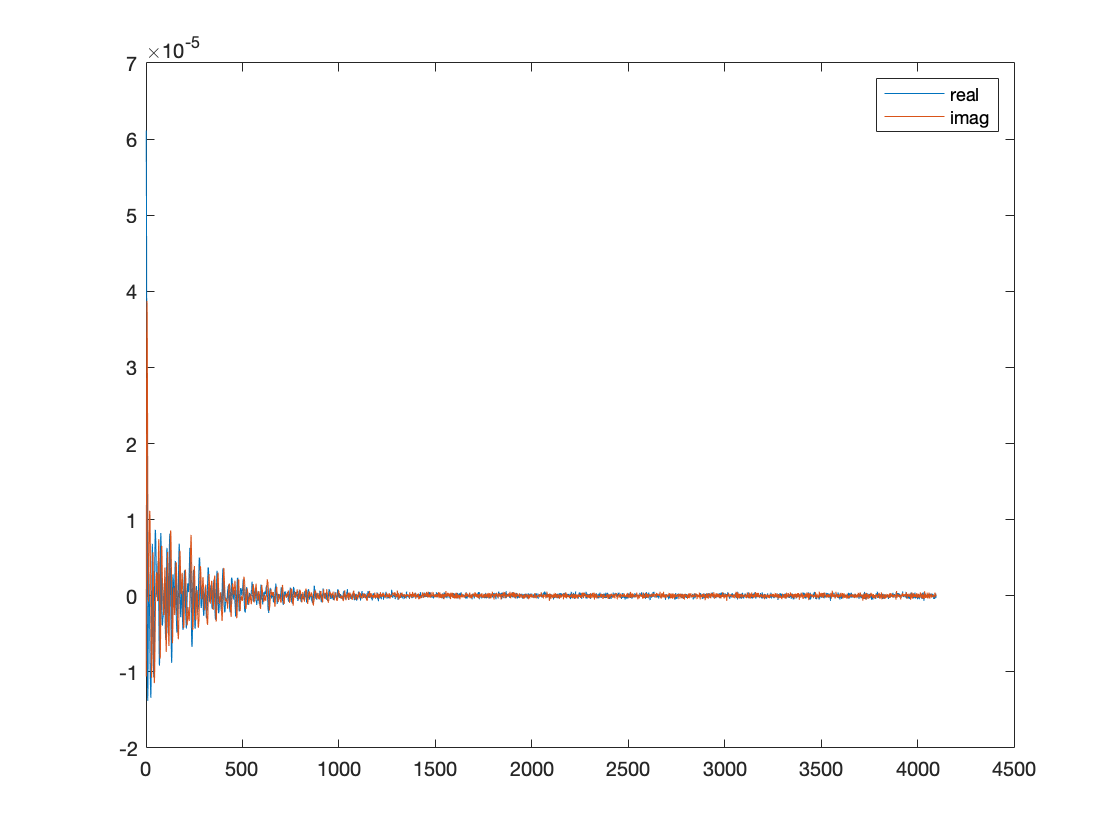
\includegraphics[width=\maxwidth{56.196688409433015em}]{figure_0}
\end{center}

\matlabheading{The NIfTI header}

\begin{par}
\begin{flushleft}
We obviously require a few bits of information to reconstruct the frequency-domain data, most notably the dwell time and the spectrometer frequency. We find the dwell time from the standard NIfTI header:
\end{flushleft}
\end{par}

\begin{matlabcode}
nii.hdr
\end{matlabcode}
\begin{matlaboutput}
ans = 
        sizeof_hdr: 540
             magic: 'n+2 ←↵'
          datatype: 32
            bitpix: 64
               dim: [4 1 1 1 4096 1 1 1]
         intent_p1: 0
         intent_p2: 0
         intent_p3: 0
            pixdim: [1 20 20 20 8.3300e-05 1 1 1]
        vox_offset: 848
         scl_slope: 1
         scl_inter: 0
           cal_max: 0
           cal_min: 0
    slice_duration: 0
           toffset: 0
       slice_start: 0
         slice_end: 0
           descrip: ''
          aux_file: ''
        qform_code: 2
        sform_code: 2
         quatern_b: 1
         quatern_c: 0
         quatern_d: 0
         qoffset_x: -32.9007
         qoffset_y: 10.6634
         qoffset_z: 21.3559
            srow_x: [20 0 0 -32.9007]
            srow_y: [0 -20 0 10.6634]
            srow_z: [0 0 -20 21.3559]
        slice_code: 0
        xyzt_units: 0
       intent_code: 0
       intent_name: 'mrs_v0_2'
          dim_info: 0
        unused_str: ''
         extension: [1 0 0 0]
           version: 2
       swap_endian: 0
         file_name: '/Users/Georg/Documents/MATLAB/mrs_nifti_standard/example_data/svs_1/svs_preprocessed.nii.gz'

\end{matlaboutput}

\begin{par}
\begin{flushleft}
We find the dwell time (in s) in the \texttt{pixdim} field of the NIfTI header, and can derive the spectral width:
\end{flushleft}
\end{par}

\begin{matlabcode}
sw = 1/nii.hdr.pixdim(5)
\end{matlabcode}
\begin{matlaboutput}
sw = 1.2005e+04
\end{matlaboutput}

\begin{par}
\begin{flushleft}
We also find the spatial coordinates of the MRS voxel (dimensions and offset) in the s\texttt{form} field, which we can use to create a voxel overlay mask on an anatomical image.
\end{flushleft}
\end{par}

\matlabheading{The NIfTI MRS header extension}

\begin{par}
\begin{flushleft}
We still require the spectrometer frequency, which is stored in the header extension. We can access this JSON-formatted bit of information as follows:
\end{flushleft}
\end{par}

\begin{matlabcode}
% Decode the JSON header extension string
header_extension = jsondecode(nii.ext.edata_decoded)
\end{matlabcode}
\begin{matlaboutput}
header_extension = 
    TransmitterFrequency: 297.2199
         ResonantNucleus: '1H'
                EchoTime: 0.0110
          RepetitionTime: 5
           InversionTime: []
              MixingTime: 0.0320
        ConversionMethod: 'Manual'
          ConversionTime: '2020-11-20T08:20:51.208'
            OriginalFile: {'meas_MID310_STEAM_metab_FID115673.dat'}

\end{matlaboutput}

\begin{par}
\begin{flushleft}
With the spectrometer frequency in MHz now known, we can create a chemical shift axis:
\end{flushleft}
\end{par}

\begin{matlabcode}
% Extract F0 and number of samples
f0 = header_extension.TransmitterFrequency;
npts = nii.hdr.dim(5);

% Create frequency axis
f = [(-sw/2)+(sw/(2*npts)):sw/(npts):(sw/2)-(sw/(2*npts))];
% Convert to ppm
ppm = -f/f0;
ppm = ppm + 4.68;

% Calculate and plot the frequency domain spectrum
spec = fftshift(fft(fid));
plot(ppm, real(spec));
hold on;
plot(ppm, imag(spec));
set(gca, 'xdir', 'reverse', 'xlim', [0 5]);
xlabel('Chemical shift (ppm)');
hold off;
\end{matlabcode}
\begin{center}
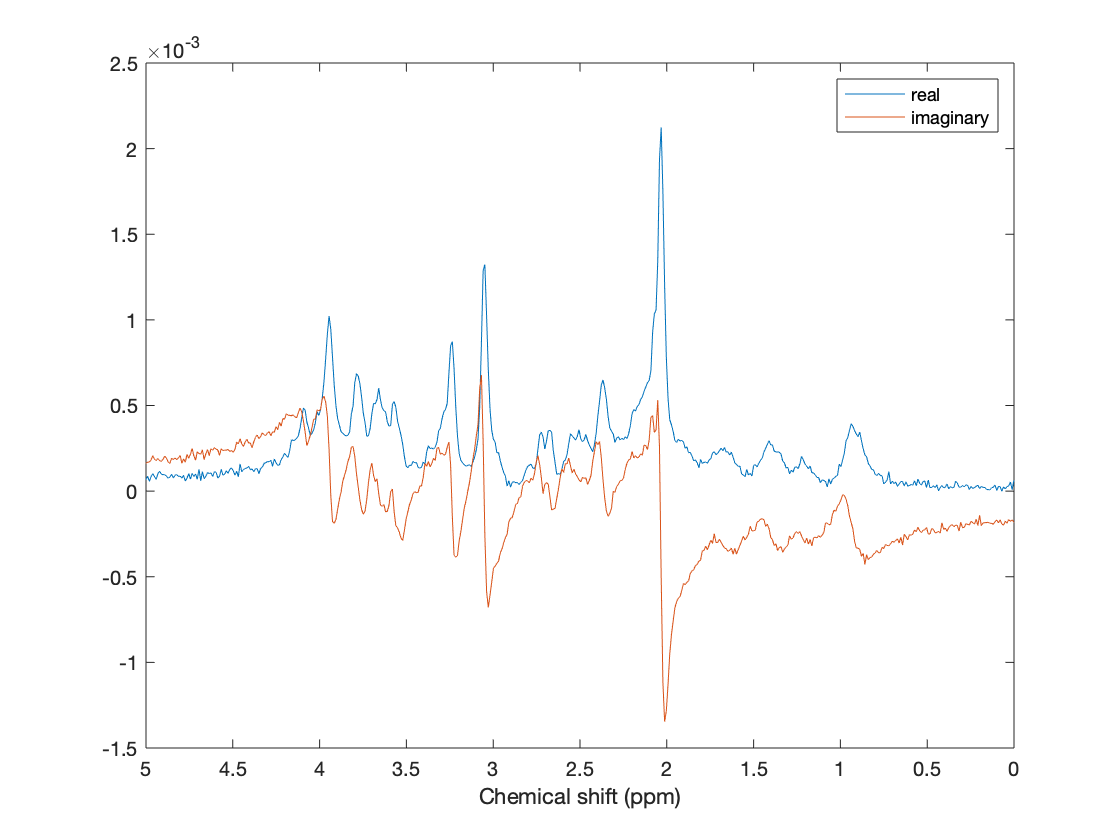
\includegraphics[width=\maxwidth{56.196688409433015em}]{figure_1}
\end{center}

\end{document}
